% !TeX program = xelatex
% Standalone Beamer source. Compile twice with XeLaTeX.
% Optional presenter view: define \DSnotes before loading this file.
% Updated 8 October 2026: public workspace, rule playback, AI switches and DS Library.
% Dated evaluations retain their original dates and denominators.
\documentclass[aspectratio=169,11pt]{beamer}
\usepackage{fontspec}
\usepackage{unicode-math}
\usepackage{booktabs,array,tabularx}
\usepackage{tikz}
\usepackage{pgfpages}
\usetikzlibrary{arrows.meta,positioning,calc,fit}

\IfFontExistsTF{Arial}{\setsansfont{Arial}}{\setsansfont{DejaVu Sans}}
\IfFontExistsTF{Menlo}{\setmonofont[Scale=0.85]{Menlo}}{\setmonofont[Scale=0.85]{DejaVu Sans Mono}}
\IfFontExistsTF{STIX Two Math}{\setmathfont{STIX Two Math}}{\setmathfont{Latin Modern Math}}
\usefonttheme{professionalfonts}

\definecolor{Ink}{HTML}{183C34}
\definecolor{Muted}{HTML}{536760}
\definecolor{Paper}{HTML}{FAFAF6}
\definecolor{Pale}{HTML}{EAF0E9}
\definecolor{Accent}{HTML}{AD592F}
\definecolor{Rule}{HTML}{CBD6CA}
\setbeamercolor{normal text}{fg=Ink,bg=Paper}
\setbeamercolor{frametitle}{fg=Ink,bg=Paper}
\setbeamercolor{structure}{fg=Ink}
\setbeamercolor{alerted text}{fg=Accent}
\setbeamercolor{block title}{fg=Ink,bg=Pale}
\setbeamercolor{block body}{fg=Ink,bg=Pale}
\setbeamerfont{frametitle}{size=\Large,series=\bfseries}
\setbeamertemplate{navigation symbols}{}
\setbeamertemplate{itemize item}{\small\textcolor{Accent}{\textbullet}}
\setbeamertemplate{itemize subitem}{\textcolor{Accent}{\textendash}}
\setbeamersize{text margin left=9mm,text margin right=9mm}
\setbeamertemplate{frametitle}{\vspace{3mm}\insertframetitle\par\vspace{1mm}}
\newif\ifDSappendix
\setbeamertemplate{footline}{%
  \hspace{9mm}\textcolor{Muted}{\scriptsize DS Workbench\quad\textbar\quad updated 8 October 2026}%
  \hfill\textcolor{Muted}{\scriptsize\ifDSappendix Appendix\enspace\fi\insertframenumber}\hspace{9mm}\vspace{3mm}}
\setbeamertemplate{note page}[plain]
\ifdefined\DSnotes
  \setbeameroption{show notes on second screen=right}
\else
  \setbeameroption{hide notes}
\fi
\hypersetup{pdftitle={DS Workbench: From Words to Transparent Meanings},
  pdfsubject={Dynamic Syntax, theoretical coverage, semantic backends, model assistance and community extension},
  colorlinks=true,urlcolor=Accent,linkcolor=Ink}

% Replace with the presenter's name if desired.
\newcommand{\DSPresenter}{}
\newcommand{\tagline}[1]{{\small\color{Accent}\bfseries #1}\par\medskip}
\newcommand{\aside}[1]{\par{\small\color{Muted}#1}\par}
\newcommand{\keypoint}[1]{\begin{block}{}#1\end{block}}
\newcommand{\code}[1]{\texttt{#1}}
\newcommand{\pred}[1]{\mathsf{#1}}
\newcommand{\source}[1]{\par\vfill{\scriptsize\color{Muted}#1}\par}
\newcolumntype{Y}{>{\raggedright\arraybackslash}X}
\tikzset{box/.style={draw=Rule,fill=Pale,rounded corners=2pt,align=center,
    inner sep=7pt,font=\small,text=Ink},
  dsstep/.style={box,minimum height=12mm},
  edge/.style={-{Stealth[length=2mm]},thick,draw=Muted},
  linkedge/.style={edge,dashed,draw=Accent},
  treenode/.style={draw=Rule,fill=white,rounded corners=2pt,inner sep=5pt,
    align=center,font=\small,text=Ink}}

\title{DS Workbench}
\subtitle{Syntax as the growth of transparent semantic representations}
\author{\DSPresenter}
\date{8 October 2026}

\begin{document}

% Slide 1
\begin{frame}[plain]
  \vspace{5mm}
  {\color{Accent}\bfseries\large $\lambda$\quad DS WORKBENCH}\par\vspace{6mm}
  {\fontsize{28}{33}\selectfont\bfseries Syntax as the growth of\\transparent semantic\\representations}\par\vspace{5mm}
  {\large An executable research workbench for Dynamic Syntax}\par\vspace{4mm}
  \aside{Classical semantics\quad /\quad Constructive semantics\quad /\quad TTR}
  \vfill
  {\small\DSPresenter\quad 8 October 2026}\par\smallskip
  \href{https://ds-workbench.vercel.app/}{\small ds-workbench.vercel.app}
  \note{Updated on 8 October against public application/source snapshot 1aff525. The community repository is now github.com/StergiosCha/DS\_workbench. This edition adds the redesigned workspace, explicit model controls, computational-rule playback and the searchable research library, alongside the earlier grammar extensions. The frozen coverage measurements retain their original dates. Present a research and teaching system with expanding fragments, not an arbitrary-text parser. A tagged workbench package release remains pending.}
\end{frame}

% Slide 2
\begin{frame}{Built with AI assistance}
  \color{Ink}
  \tagline{Development tools and model access}
  \begin{block}{Development}
    \textbf{Astra} with \textbf{Codex}\par\medskip
    \textbf{Fable 5.1} with \textbf{Claude Code}
  \end{block}
  \vspace{5mm}
  \begin{block}{Models in the application}
    \textbf{OpenRouter} provides access to all models used in the app.
  \end{block}
  \note{Development used Astra with Codex and Fable 5.1 with Claude Code. OpenRouter provides access to the models used inside the application.}
\end{frame}

% Slide 3
\begin{frame}{The research question}
  \color{Ink}
  \tagline{Can we broaden coverage while keeping derivations inspectable?}
  \begin{columns}[T,onlytextwidth]
    \column{.48\textwidth}
      \textbf{For a linguist}\medskip
      \begin{itemize}\setlength\itemsep{7pt}
        \item Which word licensed each operation?
        \item Which requirements are still open?
        \item Where did this meaning come from?
      \end{itemize}
    \column{.48\textwidth}
      \textbf{For an engineering system}\medskip
      \begin{itemize}\setlength\itemsep{7pt}
        \item Use dictionaries and corpora.
        \item Let models propose useful analyses.
        \item Retain failures and alternatives.
      \end{itemize}
  \end{columns}
  \vspace{5mm}
  \keypoint{The DS engine must build the derivation. A model suggestion is an assumption to examine.}
  \note{The motivation is the tension between a transparent formal fragment and ordinary open text. Three questions must stay separate: lexical coverage, formal completion, and linguistic adequacy. The interface is designed to expose rather than collapse them.}
\end{frame}

% Slide 4
\begin{frame}{One word changes the state}
  \color{Ink}
  \tagline{A tree, a pointer, and requirements}
  \centering
  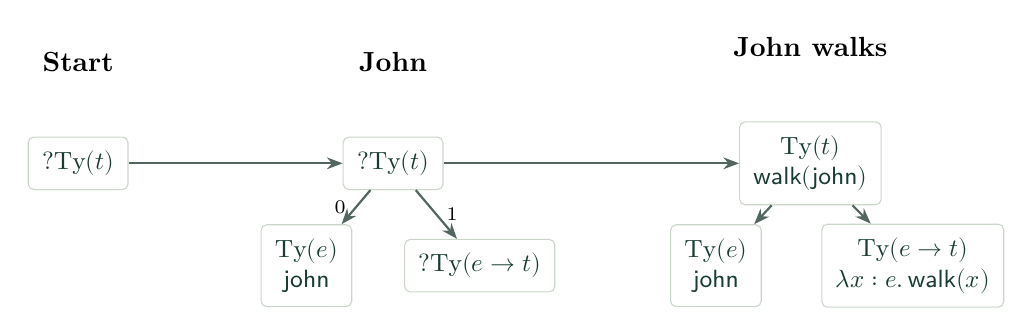
\begin{tikzpicture}[x=1cm,y=1cm]
    \node[treenode] (a) at (0,0) {$?\mathrm{Ty}(t)$};
    \node[above=7mm of a,font=\bfseries] {Start};
    \node[treenode] (b) at (4,0) {$?\mathrm{Ty}(t)$};
    \node[treenode] (b0) at (2.9,-1.3) {$\mathrm{Ty}(e)$\\$\pred{john}$};
    \node[treenode] (b1) at (5.1,-1.3) {$?\mathrm{Ty}(e\to t)$};
    \draw[edge] (b)--node[left,font=\scriptsize]{0}(b0);
    \draw[edge] (b)--node[right,font=\scriptsize]{1}(b1);
    \node[above=7mm of b,font=\bfseries] {John};
    \node[treenode] (c) at (9.3,0) {$\mathrm{Ty}(t)$\\$\pred{walk}(\pred{john})$};
    \node[treenode] (c0) at (8.1,-1.3) {$\mathrm{Ty}(e)$\\$\pred{john}$};
    \node[treenode] (c1) at (10.6,-1.3) {$\mathrm{Ty}(e\to t)$\\$\lambda x:e.\,\pred{walk}(x)$};
    \draw[edge] (c)--(c0); \draw[edge] (c)--(c1);
    \node[above=7mm of c,font=\bfseries] {John walks};
    \draw[edge] (a.east)--(b.west);
    \draw[edge] (b.east)--(c.west);
  \end{tikzpicture}\par
  \vspace{4mm}
  \aside{Schematic Classical states after local completion; intermediate pointer movements are omitted.}
  \note{Question marks represent outstanding requirements, not probabilities. Lexical and computational rules build the daughters and compose by typed application. This drawing compresses intermediate steps; the application can show the individual make, go and put instructions. The context DAG stores alternatives and is different from this one semantic tree.}
\end{frame}

% Slide 5
\begin{frame}{What the project is built on}
  \color{Ink}
  \tagline{Software foundation}
  \centering
  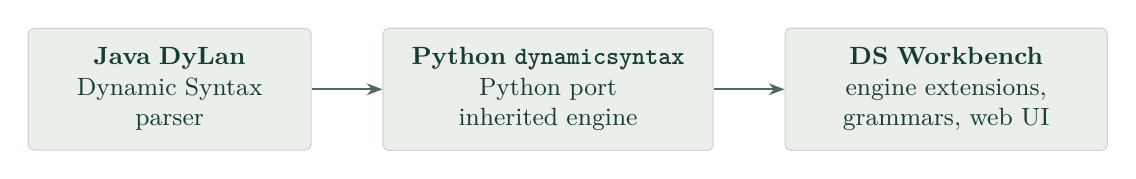
\begin{tikzpicture}
    \node[dsstep,text width=31mm] (java) {\textbf{Java DyLan}\\Dynamic Syntax\\parser};
    \node[dsstep,text width=37mm,right=9mm of java] (python) {\textbf{Python \code{dynamicsyntax}}\\Python port\\inherited engine};
    \node[dsstep,text width=36mm,right=9mm of python] (app) {\textbf{DS Workbench}\\engine extensions,\\grammars, web UI};
    \draw[edge] (java)--(python); \draw[edge] (python)--(app);
  \end{tikzpicture}\par
  \vspace{6mm}
  \begin{itemize}\setlength\itemsep{6pt}
    \item \code{dynamicsyntax}: public Python API, grammar discovery, results.
    \item \code{dylan}: most parser, tree, action and formula implementation.
    \item A DS parser with substantial TTR machinery is the foundation.
  \end{itemize}
  \note{The two Python namespaces are part of one distribution, not separate servers. Installing the published package alone does not reproduce this modified source checkout, its resources or the deployed application.}
\end{frame}

% Slide 6
\begin{frame}{What the workbench adds}
  \color{Ink}
  \small
  \begin{tabularx}{\textwidth}{@{}p{28mm}YY@{}}\toprule
    & \textbf{Inherited foundation} & \textbf{Extensions in this workbench}\\\midrule
    Parsing & Incrementality, action language, alternatives, context DAG & Recovery, limits, diagnostics, replay and state isolation\\[4pt]
    Semantics & TTR records and composition & Native Classical/Constructive terms; TTR identity corrections\\[4pt]
    Grammar & Bundled resources and induction infrastructure & English/Greek fragments; typed templates; supplemental relatives\\[4pt]
    Application & Existing interfaces and visualisation work & Focused browser views, live rule replay, research library and community source\\\bottomrule
  \end{tabularx}\par
  \vspace{4mm}
  \aside{The contribution includes changes to the engine and grammars, as well as the interface.}
  \note{Avoid implying there was no previous GUI or visualisation. The current work builds on existing interfaces too. The focus here is the present integrated workbench, not a complete history of all upstream contributions.}
\end{frame}

% Slide 7
\begin{frame}{Shared DS machinery, three semantic implementations}
  \color{Ink}
  \small
  \begin{tabularx}{\textwidth}{@{}p{28mm}YYY@{}}\toprule
    & \textbf{Classical} & \textbf{Constructive} & \textbf{TTR}\\\midrule
    Representations & Predicates, $\lambda$, $\varepsilon/\tau$ choice terms & Typed witnesses, $\Sigma/\Pi$, projections & Record types, fields and dependencies\\[5pt]
    Composition & Typed application and reduction & Application, subtyping and witness closure & Record functions, paths and record merge\\[5pt]
    Current assistance & Native English / Standard Greek & Native English / Standard Greek & No construction or vocabulary compiler in this interface\\\bottomrule
  \end{tabularx}\par
  \vspace{4mm}
  \keypoint{Selecting a backend selects its grammar and semantic operations. It does not reformat a completed TTR parse.}
  \note{The shared parser architecture does not mean identical trees, coverage or meanings. Classical common-noun restrictors and Constructive common-noun types have different internal structure. Coq export belongs to the supported Constructive path, not all three systems. The app's TTR backend supplies record meanings to the Python DS executor. This is distinct from Cooper and Larsson's TTR-DS recasting of DS states and actions inside TTR; see the dedicated appendix slide and library card CL25.}
\end{frame}

% Slide 8
\begin{frame}{The same sentence, different semantic objects}
  \color{Ink}
  \tagline{A man knows you.}
  \setlength{\abovedisplayskip}{3pt}\setlength{\belowdisplayskip}{6pt}
  \textbf{Classical}
  \[\pred{know}\bigl(\varepsilon x:e.\,\pred{man}(x),\ \pred{you}\bigr)\]
  \textbf{Constructive: witness supplied to the predicate}
  \[\Sigma p:(\Sigma x:\pred{man}.\,\top).\ \pred{know}(\pi_1(p),\pred{you})\]
  \textbf{Constructive: simplified interpretation}
  \[\Sigma x:\pred{man}.\ \pred{know}(x,\pred{you})\]
  \aside{An interpretation type is not a constructed proof that the assertion is true.}
  \note{These are the native outputs documented in the technical report; bound-variable spelling is simplified. Explain the projection: the indefinite introduces a witness package and its first component supplies the individual argument. Do not identify a Coq type-correctness check with establishing the sentence's truth.}
\end{frame}

% Slide 9
\begin{frame}{TTR keeps participant and event dependencies explicit}
  \color{Ink}
  \begin{columns}[T,onlytextwidth]
    \column{.53\textwidth}
    \[\left[\begin{array}{ll}
      x_0 &: e\\
      p_0=\pred{man}(x_0) &: t\\
      x_1=\pred{you} &: e\\
      e_0=\pred{know} &: es\\
      p_2=\pred{pres}(e_0) &: t\\
      p_5=\pred{subj}(e_0,x_0) &: t\\
      p_4=\pred{obj}(e_0,x_1) &: t\\
      \pred{head}=e_0 &: es
    \end{array}\right]\]
    \column{.43\textwidth}
    \vspace{3mm}
    \begin{itemize}\setlength\itemsep{9pt}
      \item Subject and object retain their own dependencies.
      \item Freshening must preserve constants and field identity.
      \item Native grammar extensions do not automatically extend TTR.
    \end{itemize}
  \end{columns}
  \aside{Readable presentation of the recorded TTR analysis; field equality here denotes a manifest field.}
  \note{The earlier TTR bug allowed variable collisions to corrupt argument identity even when a tree completed. Branch-local freshening, constant preservation and semantic regression tests were needed. Different variable names do not assert that the referents are unequal: they preserve dependency structure. This motivates checking meaning, not just a green badge.}
\end{frame}

% Slide 10
\begin{frame}{Coverage is a set of executable fragments}
  \color{Ink}
  \begin{columns}[T,onlytextwidth]
    \column{.49\textwidth}
      \textbf{Native English}\medskip
      \begin{itemize}\setlength\itemsep{5pt}
        \item Names, determiners and nominal constructions.
        \item Verb frames, copulas, PP arguments and modifiers.
        \item Relatives and finite clause relations.
        \item Limited questions, reflexives and dialogue repairs.
      \end{itemize}
    \column{.47\textwidth}
      \textbf{Native Standard Greek}\medskip
      \begin{itemize}\setlength\itemsep{5pt}
        \item Case-sensitive names and nominal constructions.
        \item Clitics, clusters, verb frames and selected word orders.
        \item PP goals, comparisons and finite clause relations.
        \item Other varieties have smaller reviewed fragments.
      \end{itemize}
  \end{columns}
  \vspace{2mm}\keypoint{Coverage is defined by supported constructions, not by the language label.}
  \note{Do not claim that every determiner, relative, question or word order is supported. Number, agreement, tense, aspect and discourse remain partial. The dialect and historical displays have different evidential and executable scope.}
\end{frame}

% Slide 11
\begin{frame}{A literature map now guides implementation}
  \color{Ink}
  \tagline{18 categories\quad /\quad 91 tracked topics\quad /\quad source-linked obligations}
  \small
  \begin{tabularx}{\textwidth}{@{}p{39mm}Y@{}}\toprule
    \textbf{Families in the map} & \textbf{Examples of theoretical coverage}\\\midrule
    Growth and predication & Lexical programs, nominals, scope, valency and copulas\\[4pt]
    Dependencies & Flexible order, relatives, resumption, extraction and modification\\[4pt]
    Reference and dialogue & Coordination, binding, clitics, ellipsis, repair and grounding\\[4pt]
    Clauses and variation & Auxiliaries, tense/voice, clause linkage, agreement and historical change\\[4pt]
    Computation & Learning, search, generation and semantic architectures\\\bottomrule
  \end{tabularx}\par
  \vspace{1mm}
  \keypoint{An analysis in the literature is a starting point for a program and semantic tests. It is not automatically implemented here.}
  \note{The initial citation-led coverage review on 6–7 October had 14 bibliography entries: 13 inspected artifacts and one metadata-only follow-up. The later selected-work library has 53 works and its own inspection records; these are different inventories, not competing counts. Long books and theses received targeted section review. The five rows group the eighteen categories for presentation. The map is not exhaustive. Distinguish worked analyses, reported implementations, proposals, secondary pointers and metadata from this code's independent implementation status.}
\end{frame}

% Slide 12
\begin{frame}{A searchable library connects papers to implementation}
  \color{Ink}
  \tagline{53 selected works\quad /\quad 30 source versions\quad /\quad 8 analysis cards}
  \begin{columns}[T,onlytextwidth]
    \column{.47\textwidth}
      \textbf{Find and inspect}\medskip
      \begin{itemize}\setlength\itemsep{7pt}
        \item Open the app's \textbf{DS Library} tab.
        \item Search text; filter topic and semantic framework.
        \item See review scope and publication links.
      \end{itemize}
    \column{.49\textwidth}
      \textbf{Trace an analysis}\medskip
      \begin{enumerate}\setlength\itemsep{6pt}
        \item Work and source version.
        \item Bounded claim and exact passages.
        \item DS mechanisms and semantic obligations.
        \item Backend-specific code and tests.
      \end{enumerate}
  \end{columns}
  \vspace{3mm}
  \keypoint{Most readings are partial. A bibliographic record never establishes implemented coverage.}
  \note{The app has a read-only, generated catalogue. Filtering it sends no model request and preserves the parse. The offline library in docs/research/library has the fuller version/evidence view, eight analysis cards and BibTeX/CSL exports. The 30 source versions are fingerprinted; this does not mean 30 full readings. Work, source version, bounded analysis and implementation are separate entities. A source PDF is not redistributed by the in-app catalogue. Zotero import files exist; shared-group editing and reviewed synchronization remain future work. Include semantic framework and TTR-integration tags so DS--TTR content semantics is not confused with the separate TTR-DS recasting.}
\end{frame}

% Slide 13
\begin{frame}{PP arguments and modifiers do different jobs}
  \color{Ink}
  \begin{tabularx}{\textwidth}{@{}p{48mm}Y@{}}\toprule
    \textbf{Sentence} & \textbf{Implemented treatment}\\\midrule
    John relies \alert{on Mary}. & Selected verb argument: an \emph{on}-complement is required.\\[6pt]
    John gives a book \alert{to Mary}. & Recipient argument in the dative-to frame.\\[6pt]
    John walks \alert{in a park}. & Modifier grows through LINK; its own NP is parsed.\\[6pt]
    A man is \alert{in a park}. & Copular locative predicate.\\\bottomrule
  \end{tabularx}\par
  \vspace{4mm}
  \[\pred{in\_location}(\pred{place},\pred{walk}(\pred{john}))\]
  \aside{Schematic modifier meaning. The fragment does not supply a spatial or event-inference model.}
  \note{Address the common intuition that modifiers should be LINK structures: these PP modifiers do use LINK. Selected arguments are different. A location PP cannot silently fill a missing recipient or selected preposition requirement. These are implementation choices within this fragment, not a claim that one analysis is the only possible DS treatment.}
\end{frame}

% Slide 14
\begin{frame}{The same LINK mechanism can compose different meanings}
  \color{Ink}
  \begin{tabularx}{\textwidth}{@{}p{32mm}YY@{}}\toprule
    \textbf{Construction} & \textbf{Example} & \textbf{Semantic obligation}\\\midrule
    Restrictive relative & A man who Mary knows walks. & Refine the nominal restrictor before quantification.\\[7pt]
    Nonrestrictive relative & John, who Mary knows, walks. & Preserve John; add a supplemental assertion.\\[7pt]
    PP modifier & John walks in a park. & Attach the locative content at the intended scope.\\\bottomrule
  \end{tabularx}\par
  \vspace{3mm}
  \keypoint{Specify what is copied, where requirements close, and how the linked content is evaluated.}
  \source{Cann, Kempson \& Marten (2005), ch.3; Howes \& Gibson (2021), §§2.1, 2.5.1.}
  \note{The LINK relation is a structural resource, not a universal instruction to conjoin. The current PP treatment is the workbench's declared implementation choice. The nonrestrictive follows the source's initial conjunctive account, which is not a complete theory of projection or conventional implicature. The Classical and Constructive compilers must each satisfy the intended identity and scope contract; TTR requires its own audit.}
\end{frame}

% Slide 15
\begin{frame}{From the source analysis to an executable relative}
  \color{Ink}
  \tagline{John, who Mary knows, walks.\quad No LLM needed.}
  \begin{columns}[c,onlytextwidth]
    \column{.53\textwidth}
      \centering
      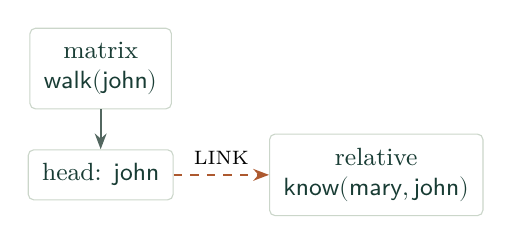
\begin{tikzpicture}[x=1cm,y=1cm]
        \node[treenode] (m) at (0,0) {matrix\\$\pred{walk}(\pred{john})$};
        \node[treenode] (h) at (0,-1.35) {head: $\pred{john}$};
        \node[treenode] (r) at (3.5,-1.35) {relative\\$\pred{know}(\pred{mary},\pred{john})$};
        \draw[edge] (m)--(h);
        \draw[linkedge] (h)--node[above,font=\scriptsize]{LINK}(r);
      \end{tikzpicture}\par
      \aside{Schematic: functor branches and intermediate states omitted.}
    \column{.43\textwidth}
      \begin{enumerate}\setlength\itemsep{6pt}
        \item Comma opens a LINKed proposition.
        \item \emph{Who} copies the head to an unfixed node.
        \item MERGE fixes the copy as the object of \emph{knows}.
        \item Close the relative; return and compose.
      \end{enumerate}
  \end{columns}
  \vspace{3mm}
  \[\pred{walk}(\pred{john})\ \wedge\ \pred{know}(\pred{mary},\pred{john})\]
  \source{Cann, Kempson \& Marten, §3.1, rules (3.6), (3.9), (3.13); inspected draft PDF pp.84–90.}
  \note{The matrix head at 00 links into 00L. Who copies its referent to L*, and the existing merge-relative rule fixes that copy at the relative subject L0 or object L10; here it is the object. Closing comma checks the relative and returns to the head. Completion-time evaluation conjoins the propositions after matrix composition. The head remains the same constant. The graphic is a compressed dependency schematic, not a screenshot or a full binary derivation. Both native backends produce the displayed formula. Classical follows the cited conjunction analysis; the Constructive typed conjunction/witness treatment is our implementation adaptation, not a claim that the source provided that exact code.}
\end{frame}

% Slide 16
\begin{frame}{Test the relative's meaning and its boundaries}
  \color{Ink}
  \begin{columns}[T,onlytextwidth]
    \column{.48\textwidth}
      \textbf{Implemented in both native English backends}\medskip
      \begin{itemize}\setlength\itemsep{6pt}
        \item Named subject or direct-object hosts.
        \item Subject or direct-object gaps.
        \item Local negation, adverbs and indefinite witnesses.
      \end{itemize}
    \column{.48\textwidth}
      \textbf{Still outside this claim}\medskip
      \begin{itemize}\setlength\itemsep{6pt}
        \item Quantified or complex definite hosts.
        \item Nonlocal gaps and embedded projection.
        \item Greek relatives and TTR parity.
      \end{itemize}
  \end{columns}
  \vspace{4mm}
  \keypoint{56 focused tests; 8 public browser checks: six complete derivations and two expected incomplete cases.}
  \aside{7 October: authored construction checks, not an estimate of unseen-text accuracy.}
  \note{The tests check exact formulas, head identity, roles, local witness scope, LINK/unfixed/MERGE operations, alternatives and Coq exports when the compiler is available. The two negative public checks use John, who Mary walks, arrives: there is no compatible object gap. They are implementation contrasts, not independently elicited judgments. Who/which animacy is not yet enforced. Polar questions, causal/temporal/conditional combinations and attitudes require a projection account before support can be claimed. The public record is data/coverage/nonrestrictive-public-2026-10-07.json, with no model calls.}
\end{frame}

% Slide 17
\begin{frame}{Greek clitics: order, case and tree growth}
  \color{Ink}
  \tagline{της τον έδωσε.\quad “S/he gave him to her.”}
  \begin{columns}[T,onlytextwidth]
    \column{.49\textwidth}
      \begin{itemize}\setlength\itemsep{8pt}
        \item Genitive recipient and accusative theme.
        \item Unfixed structure, MERGE and substitution.
        \item Ditransitive frame preserves three participants.
      \end{itemize}
    \column{.47\textwidth}
      \begin{block}{Readable role structure}
        \[\pred{give}(\pred{pro},\pred{him},\pred{her})\]
        \small subject\quad theme\quad recipient
      \end{block}
      \aside{Predicate renamed for readability; pronoun reference is assumed.}
  \end{columns}
  \vspace{3mm}
  \keypoint{PCC control: \emph{του με έδωσε} fails in the modeled SMG clitic reading, in both native backends.}
  \note{The formula renames the generated predicate while preserving roles. Genitive needs a recipient slot; a transitive lexical entry previously left it unresolved. The PCC card links Chatzikyriakidis's thesis entry (6.49) and the 2011 article: genitive and first/second-person accusative programs compete for a locally unfixed address, while third-person accusatives have a fixed strategy. An unfixed node in a prefix is legitimate; the full PCC cluster must not receive a complete result. The user-supplied control is a regression example, not an independently sourced sentence judgment or a restriction generalized to all dialects and strong pronouns. Corpus frames remain hypotheses. Historical panels are not executable historical grammars.}
\end{frame}

% Slide 18
\begin{frame}{What already works without an LLM}
  \color{Ink}
  \centering
  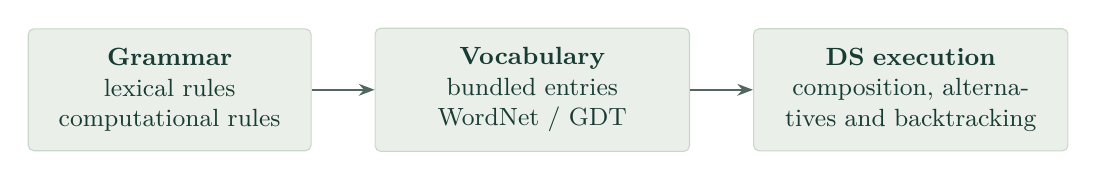
\begin{tikzpicture}
    \node[dsstep,text width=31mm] (g) {\textbf{Grammar}\\lexical rules\\computational rules};
    \node[dsstep,text width=35mm,right=8mm of g] (v) {\textbf{Vocabulary}\\bundled entries\\WordNet / GDT};
    \node[dsstep,text width=35mm,right=8mm of v] (d) {\textbf{DS execution}\\composition, alternatives and backtracking};
    \draw[edge] (g)--(v); \draw[edge] (v)--(d);
  \end{tikzpicture}\par
  \vspace{6mm}
  \begin{itemize}\setlength\itemsep{6pt}
    \item Tree growth, meaning composition, diagnostics and playback.
    \item Sentence, paragraph and supported dialogue flows.
    \item Corpus/dictionary investigation and exports.
  \end{itemize}
  \keypoint{A model key is optional. Dictionaries still supply candidates, not guaranteed contextual meanings.}
  \note{In dictionary or corpus mode there is no lexical model request. Corpus investigation may involve a live source service, but that is not an LLM call. A fully supported sentence can complete without a model in assisted mode too, except that ambiguous connective selection may deliberately request a contextual preference.}
\end{frame}

% Slide 19
\begin{frame}{From the browser to an isolated DS worker}
  \color{Ink}
  \centering
  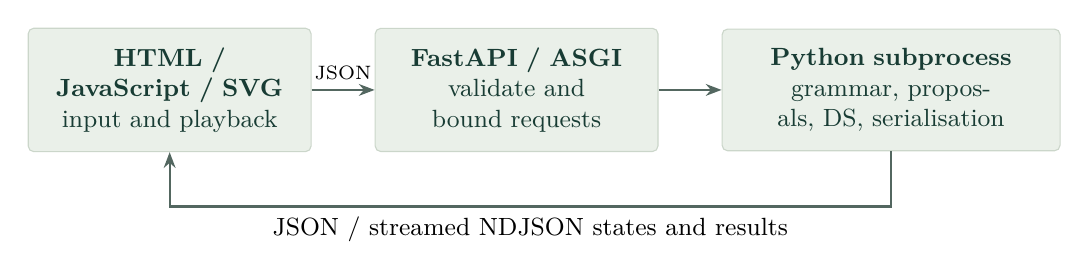
\begin{tikzpicture}
    \node[dsstep,text width=31mm] (ui) {\textbf{HTML / JavaScript / SVG}\\input and playback};
    \node[dsstep,text width=31mm,right=8mm of ui] (api) {\textbf{FastAPI / ASGI}\\validate and bound requests};
    \node[dsstep,text width=38mm,right=8mm of api] (w) {\textbf{Python subprocess}\\grammar, proposals, DS, serialisation};
    \draw[edge] (ui)--node[above,font=\scriptsize]{JSON}(api);
    \draw[edge] (api)--(w);
    \draw[edge] (w.south)--++(0,-.7)-|node[below,pos=.25,font=\small]{JSON / streamed NDJSON states and results}(ui.south);
  \end{tikzpicture}\par
  \vspace{10mm}
  \begin{itemize}\setlength\itemsep{6pt}
    \item Process isolation protects mutable parser and metavariable state.
    \item The browser renders recorded states; it does not run the parser.
  \end{itemize}
  \note{The local standard-library HTTP server and hosted ASGI application use the same parser API. Request, response, worker and concurrency limits are part of deployment. The model key stays in the tab until refresh/disconnect, travels through the DS server for requests, and is not saved by the app. Avoid claiming that process isolation itself proves the implementation correct.}
\end{frame}

% Slide 20
\begin{frame}{The model and the engine have distinct responsibilities}
  \color{Ink}
  \begin{tabularx}{\textwidth}{@{}p{30mm}YY@{}}\toprule
    & \textbf{Selected chat model} & \textbf{DS engine and compiler}\\\midrule
    Vocabulary & Propose lemma, sense, morphology and argument frame & Validate fields and instantiate an allowed lexical template\\[5pt]
    Constructions & Select a declared clause relation; propose a connective use & Instantiate a reviewed construction and compose its contents\\[5pt]
    Failure & Revise a hypothesis using actual DS feedback & Retry within limits; retain incomplete results\\\bottomrule
  \end{tabularx}\par
  \vspace{3mm}
  \keypoint{Model output contains structured hypotheses. It does not contain executable code or a finished replacement tree.}
  \note{This is the central architectural change. Previously the model could only propose content words; conjunctions were excluded. The new interface supports construction hypotheses while keeping the underlying grammar operations reviewed. A model may still propose the wrong interpretation even if every schema and type check passes.}
\end{frame}

% Slide 21
\begin{frame}{Two switches choose what the next parse may use}
  \color{Ink}
  \tagline{Use analysis LLM\qquad /\qquad Use Jev}
  \small
  \begin{tabularx}{\textwidth}{@{}p{17mm}p{17mm}Y@{}}\toprule
    \textbf{LLM} & \textbf{Jev} & \textbf{Enabled route}\\\midrule
    OFF & OFF & DS with the selected original, bundled, dictionary or corpus vocabulary.\\[6pt]
    ON & OFF & Bounded lexical and construction assistance when needed.\\[6pt]
    OFF & ON & Jev word-meaning preferences; no generative fallback.\\[6pt]
    ON & ON & Jev preferences plus lexical-model fallback; no construction assistance in this combined mode.\\\bottomrule
  \end{tabularx}\par
  \vspace{3mm}
  \normalsize\keypoint{\textbf{Connect / models} sets up access. The switches authorize use.\par
    \textbf{This result} reports the requests actually made.}
  \note{Both switches default off. Connecting or choosing a model does not enable either, and switching does not start a parse. An enabled LLM can make zero calls when the available grammar is sufficient. The result counters describe the displayed parse even if the settings change afterward. Jev sense assistance is native-English only; neither model assists TTR here. English dialogue supports lexical proposals, not open-text construction assistance. Jev's advanced search-order control is distinct and still calibration-gated; Turn off all AI also resets it. No key is needed for grammar-only work. Model calls use the visitor's OpenRouter account, and input goes to the selected provider.}
\end{frame}

% Slide 22
\begin{frame}{A construction family replaces one-off conjunction fixes}
  \color{Ink}
  \tagline{Surface word $\longrightarrow$ declared relation $\longrightarrow$ shared DS program}
  \begin{tabularx}{\textwidth}{@{}p{34mm}YY@{}}\toprule
    \textbf{Family} & \textbf{English examples} & \textbf{Greek examples}\\\midrule
    Cause & because; causal since & επειδή, διότι; causal αφού\\[4pt]
    Time & when, while, before, after, until & όταν, όποτε, ωσότου\\[4pt]
    Condition & if, unless & αν, εάν\\[4pt]
    Concession /\newline contrast & although, though, whereas & παρότι, μολονότι; readings of ενώ\\\bottomrule
  \end{tabularx}\par
  \vspace{4mm}
  \aside{Postposed clauses grow through LINK. Fronted clauses require an explicit comma and a main clause. Ambiguous words retain alternatives.}
  \note{There are twelve relation IDs, not one generic conjunction that erases distinctions. The model can choose among declared readings or add a previously absent single-word lexicalization. The table lists supported finite-clause uses only: nominal after, interrogative when, multiword markers and nonfinite complements are not licensed by these templates.}
\end{frame}

% Slide 23
\begin{frame}{A recorded example of model assistance}
  \color{Ink}
  \tagline{John walks provided Mary walks.}
  \begin{columns}[T,onlytextwidth]
    \column{.46\textwidth}
      \textbf{Before assistance}\medskip
      \aside{The available lexical programs do not license this connective use.}
      \medskip\textbf{Model proposal}\medskip
      \begin{block}{}\code{surface: provided}\\\code{relation: condition}\end{block}
    \column{.5\textwidth}
      \textbf{Actual DS result}\medskip
      \[\begin{aligned}
        \pred{condition}(&\pred{walk}(\pred{john}),\\[-1mm]
                         &\pred{walk}(\pred{mary}))
      \end{aligned}\]
      \aside{The UI exposes the compiled template and the relation on the accepted DS path.}
  \end{columns}
  \vspace{3mm}
  \keypoint{Recorded 4 October checks: \emph{provided} and Greek \emph{καθότι} completed in both native backends.}
  \note{These were real OpenRouter calls followed by DS parsing, recorded on 4 October, not new calls made for this slide update. For καθότι, the missing-word request returned a construction directly instead of exhausting the retry budget on noun/verb guesses. The public browser check also verified provided, export and key privacy. These demonstrations do not estimate general model accuracy.}
\end{frame}

% Slide 24
\begin{frame}{Jev has a different, visible role}
  \color{Ink}
  \tagline{John lends a book to Mary.}
  \begin{columns}[T,onlytextwidth]
    \column{.48\textwidth}
      \begin{block}{DS without Jev preferences}
        \textbf{“bestow a quality on”}\medskip
        \aside{A complete but contextually poor lexical-sense choice.}
      \end{block}
    \column{.48\textwidth}
      \begin{block}{DS with Jev preferences}
        \textbf{“give temporarily”}\medskip
        \aside{DS replay accepts a preferred sense after more context arrives.}
      \end{block}
  \end{columns}
  \vspace{4mm}
  \begin{itemize}\setlength\itemsep{6pt}
    \item Two actual runs use identical lexical programs.
    \item Jev ranks senses from the observed prefix; alternatives survive.
    \item Its pinned model is separate from the selected chat model.
  \end{itemize}
  \source{Recorded demonstration, not an accuracy or speed benchmark. The independent search-order control remains gated by calibration.}
  \note{Show the distinction between semantic adequacy and formal completion: both parses completed. Jev's early response may be uncertain and outcomes vary across calls. The controlled comparison freezes candidates and semantic profiles; simply switching dictionary modes would not be a fair comparison because their candidate order differs. Comparison currently supports native English sentences only.}
\end{frame}

% Slide 25
\begin{frame}{Corpora and dictionaries supply evidence}
  \color{Ink}
  \begin{columns}[T,onlytextwidth]
    \column{.47\textwidth}
      \textbf{Lexical resources}\medskip
      \begin{itemize}\setlength\itemsep{6pt}
        \item English: reviewed additions; optional WordNet index.
        \item Greek: GDT training export.
        \item 2,021 Greek forms; 2,330 analyses.
      \end{itemize}
    \column{.49\textwidth}
      \textbf{Optional live Greek evidence}\medskip
      \begin{itemize}\setlength\itemsep{6pt}
        \item Svarna examples and corpus context.
        \item Triantafyllidis headwords and excerpts.
        \item Observations and citations accompany lexical proposals.
      \end{itemize}
  \end{columns}
  \vspace{5mm}
  \keypoint{An attested occurrence is evidence for an analysis. It is not an exhaustive valency specification or automatic grammar training.}
  \note{Live parsing integration is opt-in and bounded, for native Standard Greek sentence/paragraph assistance. Retrieved IDs are validated, but citation relevance is not automatically proven. Held-out GDT material is separate from the training builder. Explain the independent source licenses if the audience asks about redistribution.}
\end{frame}

% Slide 26
\begin{frame}{Sentences, paragraphs and dialogue}
  \color{Ink}
  \begin{tabularx}{\textwidth}{@{}p{27mm}YY@{}}\toprule
    \textbf{Input} & \textbf{State handling} & \textbf{Important boundary}\\\midrule
    Sentence & Incremental parse and alternative complete analyses & Completion is relative to the selected grammar\\[6pt]
    Paragraph & Completed sentences retain DS context & Failures count and become explicit context gaps\\[6pt]
    Dialogue & A new speaker can continue the same tree; supported repairs preserve history & General ellipsis, grounding and discourse inference remain incomplete\\\bottomrule
  \end{tabularx}\par
  \vspace{5mm}
  \aside{A later successful sentence does not turn an incomplete paragraph into a complete interpretation.}
  \note{The interface supports up to 400 paragraph tokens and 24 sentences, and up to 12 dialogue turns and 80 tokens. Basic name-based pronoun resolution is not a general discourse model. Open-text construction assistance applies to sentences and paragraphs; it is not the dialogue assistance pipeline.}
\end{frame}

% Slide 27
\begin{frame}{A workspace organised around the growing tree}
  \color{Ink}
  \centering
  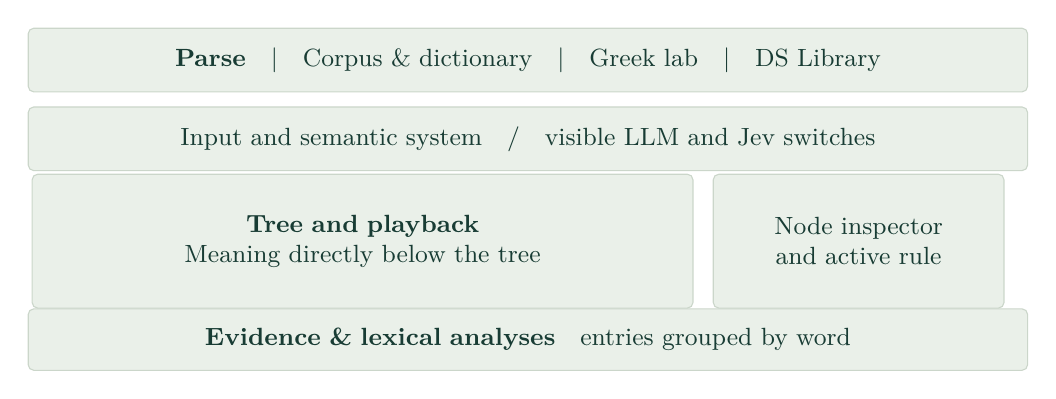
\begin{tikzpicture}[x=1cm,y=1cm]
    \node[box,text width=122mm,minimum height=7mm] at (0,0)
      {\textbf{Parse}\quad |\quad Corpus \& dictionary\quad |\quad Greek lab\quad |\quad DS Library};
    \node[box,text width=122mm,minimum height=8mm] at (0,-1.0)
      {Input and semantic system\quad /\quad visible LLM and Jev switches};
    \node[box,text width=79mm,minimum height=17mm] at (-2.1,-2.3)
      {\textbf{Tree and playback}\\Meaning directly below the tree};
    \node[box,text width=32mm,minimum height=17mm] at (4.2,-2.3)
      {Node inspector\\and active rule};
    \node[box,text width=122mm,minimum height=7mm] at (0,-3.55)
      {\textbf{Evidence \& lexical analyses}\quad entries grouped by word};
  \end{tikzpicture}\par
  \vspace{3mm}
  \aside{Settings open in a drawer. Tabs preserve the parse. Manual zoom persists; Auto-fit resumes following the tree.}
  \note{This is a layout schematic, not an application screenshot. The new desktop view places the tree closer to input. Three examples are shown initially; All examples expands them. Parse options and coverage are a disclosure. On mobile, larger playback targets and a wrapping timeline keep controls accessible; meaning stays below the tree and Inspect this step opens the inspector. A node click pauses playback and opens its details. Evidence follows the tree, with candidate programs grouped by word and reported selections first. Inspect failure opens the evidence. Tabs alone make no parser/model request; asking DS to analyse a corpus or Greek-lab example returns to Parse. Fullscreen and side-by-side semantic comparison are not implemented by this redesign.}
\end{frame}

% Slide 28
\begin{frame}{Computational rules appear while the tree grows}
  \color{Ink}
  \tagline{Rules is the default playback level}
  \begin{columns}[T,onlytextwidth]
    \column{.48\textwidth}
      \textbf{See the active program}\medskip
      \begin{itemize}\setlength\itemsep{6pt}
        \item Lexical and computational rules in execution order.
        \item Introduction and anticipation; completion and elimination.
        \item Pointer movement and changed decorations.
      \end{itemize}
    \column{.48\textwidth}
      \textbf{Choose the level of detail}\medskip
      \begin{itemize}\setlength\itemsep{6pt}
        \item \textbf{Words}: states at word boundaries.
        \item \textbf{Rules}: each lexical/computational action.
        \item \textbf{Operations}: make/go/put inside a rule, where recorded.
      \end{itemize}
  \end{columns}
  \vspace{2mm}
  \keypoint{Backtracking restores a prior state. \textbf{Show final result} returns to the endpoint.}
  \note{In the current grammar, intro-pred combines Introduction/Prediction by creating argument and predicate daughters with type requirements. Anticipation0/1 separately move the pointer to children with open requirements. These are DS grammar actions, not model predictions; names and schedules differ across grammars. Rule-level events are emitted as parsing advances for ordinary, assisted and paragraph paths; the browser replays recorded states. This is not a debugger over every rejected branch. Assisted retries restart at a labelled axiom; paragraph rows have independent traces. Ordinary sentence/dialogue traces can show atomic instructions, while assisted/paragraph traces use compact rule-level snapshots. Bounded hosted traces may make an explicitly labelled jump to the final state. A partial playback frame does not contradict a complete final result. JSON and supported Constructive Coq export remain available; the public server does not execute Coq.}
\end{frame}

% Slide 29
\begin{frame}{Evidence for coverage: keep the samples separate}
  \color{Ink}
  \small
  \begin{tabularx}{\textwidth}{@{}p{56mm}YY@{}}\toprule
    \textbf{Check} & \textbf{English} & \textbf{Greek}\\\midrule
    Unseen-source baseline (1 Oct.) & 0/6 paragraphs & 0/6 passages\\[5pt]
    Hand-written assisted development set & 6/9 sentences & 5/9 sentences\\[5pt]
    New clause paragraphs & 3/3 sentences & 3/3 sentences\\[5pt]
    Live new-connective examples & provided completed & καθότι completed\\\bottomrule
  \end{tabularx}\par
  \vspace{4mm}
  \normalsize\begin{itemize}\setlength\itemsep{5pt}
    \item Results above were checked in both native backends.
    \item The frozen baseline predates the latest extensions.
    \item These small samples are not a representative accuracy estimate.
  \end{itemize}
  \note{The old unseen-source baseline is intentionally retained rather than silently replaced by successful demos. Greek passages group three consecutive test sentences; original paragraph boundaries were unavailable. The new three-sentence examples use dictionaries/corpus candidates without an LLM. Tests of known examples establish regression behavior, not open-text coverage.}
\end{frame}

% Slide 30
\begin{frame}{What “complete” does—and does not—establish}
  \color{Ink}
  \begin{columns}[T,onlytextwidth]
    \column{.47\textwidth}
      \textbf{It establishes}\medskip
      \begin{itemize}\setlength\itemsep{8pt}
        \item A path through the implemented DS programs.
        \item Satisfied tree requirements and available type checks.
        \item A composed meaning under displayed assumptions.
      \end{itemize}
    \column{.49\textwidth}
      \textbf{It does not establish}\medskip
      \begin{itemize}\setlength\itemsep{8pt}
        \item Correct sense, reference or attachment.
        \item Independent grammaticality or truth.
        \item Full temporal, causal or counterfactual reasoning.
      \end{itemize}
  \end{columns}
  \vspace{4mm}
  \keypoint{Clause relations are distinct, typed, opaque predicates. That is useful structure, but still a limited semantics.}
  \note{Condition(main, subordinate) is not silently treated as material implication. A later modifier once erased a nested clause in an alternative reading; the regression check had to assert the actual formula, not only completion. Type systems help expose errors but do not prove this Python implementation or its grammar correct.}
\end{frame}

% Slide 31
\begin{frame}{A resource other DS researchers can use and extend}
  \color{Ink}
  \begin{tabularx}{\textwidth}{@{}p{29mm}YY@{}}\toprule
    \textbf{Starting point} & \textbf{What is available} & \textbf{A useful contribution}\\\midrule
    Explore / teach & Browser, traces, examples and slides & An exercise or sourced counterexample\\[6pt]
    Reproduce & Local install, Python API, exported results & Pinned input, grammar and expected meaning\\[6pt]
    Extend & Independent grammar folders and a tested tutorial & A lexical entry or a construction family\\[6pt]
    Maintain & Builders, tests, guides and packaging checks & Review, releases and language-specific stewardship\\\bottomrule
  \end{tabularx}\par
  \vspace{4mm}
  \keypoint{The app and grammar tutorial work without a model subscription or the original developer's machine.}
  \note{Source, issues and pull requests are at github.com/StergiosCha/DS\_workbench. The public snapshot preserves inherited history and adds the workbench implementation. The community guide separates practical use, linguistic evidence, grammar work and maintenance. The wheel includes static assets and selected runtime data; clean installation outside the checkout passed HTTP/streaming and tutorial checks. Large WordNet/corpus indexes remain optional. Source publication is complete; a tagged workbench package, contributor terms and broader maintainer responsibilities remain future work. Installing the upstream PyPI package by name does not give this snapshot.}
\end{frame}

% Slide 32
\begin{frame}{Next: extend families, then measure generalisation}
  \color{Ink}
  \begin{enumerate}\setlength\itemsep{8pt}
    \item \textbf{Reference and relatives.} Source a Greek \emph{που} fragment; audit TTR identity and roles; specify supplement projection.
    \item \textbf{Predicate reuse and ellipsis.} \emph{John knows Mary. Bill does too.} Test antecedents and strict/sloppy readings.
    \item \textbf{Nominals and events.} Coordination, possessives and plurality; then auxiliaries/voice with explicit event semantics.
    \item \textbf{Community and evaluation.} Review analysis cards, tag a release, freeze fresh English/Greek samples and publish all outcomes.
  \end{enumerate}
  \vspace{2mm}\aside{Each extension needs positive examples, negative contrasts, meaningful output checks and reproducible evidence.}
  \note{These priorities follow the literature map. The first bounded English nonrestrictive increment is implemented; the Greek relative, broader ellipsis, nominal and event work listed here is future work. Ellipsis needs an accessible typed predicate history and freshening before a model can rank compatible antecedents. The full programme also includes questions, agreement, clause semantics and wider typology. Reevaluate on a fresh held-out sample; do not train on failed baseline examples and continue calling them unseen. Each backend has its own semantic obligations.}
\end{frame}

% Slide 33
\begin{frame}{A short demonstration}
  \color{Ink}
  \tagline{\href{https://ds-workbench.vercel.app/}{Open DS Workbench}\quad /\quad start in Parse}
  \begin{enumerate}\setlength\itemsep{7pt}
    \item \textbf{Without AI}\quad John, who Mary knows, walks.\\
      {\small Leave both switches OFF; follow Rules, LINK and MERGE.}
    \item \textbf{Construction assistance}\quad John walks provided Mary walks.\\
      {\small Connect privately; LLM ON, Jev OFF. Inspect the relation and actual usage.}
    \item \textbf{Jev comparison}\quad John lends a book to Mary.\\
      {\small LLM OFF, Jev ON; open \emph{See Jev in action} and compare.}
    \item \textbf{Find the research}\quad DS Library $\to$ search PCC or CL25.\\
      {\small Inspect review scope; return to Parse with the derivation preserved.}
  \end{enumerate}
  \note{Allow four to six minutes. Use native English and Classical or Constructive. The relative uses bundled original entries; to force Original lexicon use Connect / models, Advanced, Vocabulary source, then close the drawer. Step in Rules, expand a formula and show the final result. John, who Mary walks, arrives is an incomplete control. For provided enable only the analysis LLM: combining both switches selects a different lexical route without construction assistance. For lends enable only Jev and open the comparison below the evidence area, or use See Jev in action. Do not expose an API key on the projector. No new live model evaluation was run for this slide update: if the provider is unavailable, use the recorded demonstrations and identify them as recorded. The library needs no model or key.}
\end{frame}

\appendix
\DSappendixtrue

% Slide 34
\begin{frame}{Appendix: DS--TTR and TTR-DS are different proposals}
  \color{Ink}
  \small
  \begin{tabularx}{\textwidth}{@{}p{30mm}YY@{}}\toprule
    & \textbf{DS--TTR content semantics} & \textbf{TTR-DS recasting}\\\midrule
    What TTR represents & Semantic records, fields and dependencies in DS processing & DS tree descriptions, parse states and action rules themselves\\[7pt]
    In this workbench & Inherited record-semantic machinery in a Python executor & Research card and prototype specification as future work\\[7pt]
    What follows & A separate TTR grammar must be tested on its own & The existing TTR dropdown is not an implementation of this recasting\\\bottomrule
  \end{tabularx}\par
  \vspace{3mm}
  \normalsize\keypoint{A representation of DS in TTR does not require every semantic content to be a TTR record.}
  \source{Cooper \& Larsson (2025), §§1--2.2, 3, 4.8--5; DS Library record CL25 and linked analysis card.}
  \note{The inspected proposal concentrates on classical e/t contents while representing the surrounding DS machinery in TTR. Further semantic integrations and a detailed implemented grammar are left as future work. Do not read the title as evidence of a new implemented backend or of parity with Classical and Constructive. Selected sections were inspected, not every formal rule. The library keeps this distinction in a separate TTR-integration facet. An experimental prototype would require its own state/action specification and semantic regression tests before integration into the app.}
\end{frame}

% Slide 35
\begin{frame}{Appendix: bounded proposal–compile–parse loop}
  \color{Ink}
  \centering
  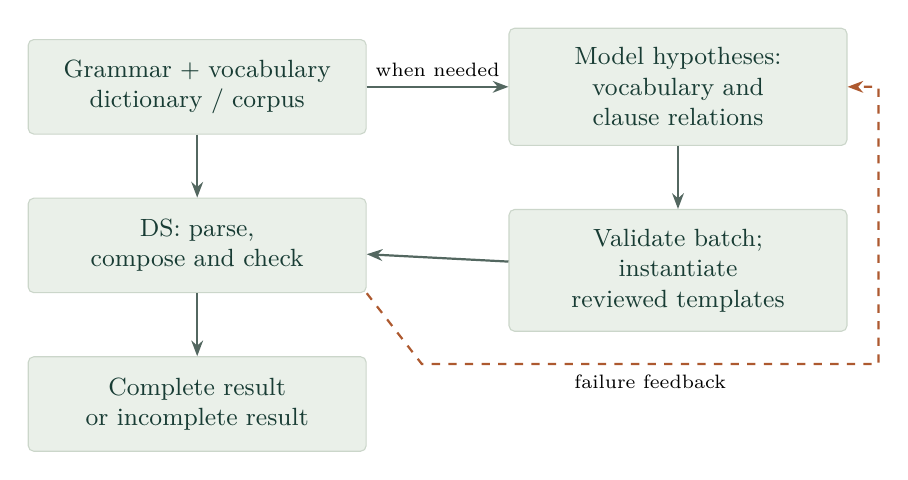
\begin{tikzpicture}[node distance=6mm]
    \node[dsstep,text width=38mm] (v) {Grammar + vocabulary\\dictionary / corpus};
    \node[dsstep,text width=38mm,right=18mm of v] (m) {Model hypotheses:\\vocabulary and\\clause relations};
    \node[dsstep,text width=38mm,below=8mm of m] (c) {Validate batch;\\instantiate\\reviewed templates};
    \node[dsstep,text width=38mm,below=8mm of v] (p) {DS: parse,\\compose and check};
    \node[dsstep,text width=38mm,below=8mm of p] (r) {Complete result\\or incomplete result};
    \draw[edge] (v)--(p);
    \draw[edge] (v)--node[above,font=\scriptsize]{when needed}(m);
    \draw[edge] (m)--(c); \draw[edge] (c)--(p);
    \draw[edge] (p)--(r);
    \draw[linkedge] (p.south east)--++(.7,-.9)--++(5.8,0)
      node[midway,below,font=\scriptsize]{failure feedback}
      |- (m.east);
  \end{tikzpicture}\par
  \vspace{3mm}
  \aside{At most three model calls, shared across a paragraph; 48-second helper budget. Provider failures preserve available grammar alternatives.}
  \note{Construction-only calls have a 16-second ceiling, vocabulary calls up to 22 seconds within remaining time. The worker boundary is 55 seconds and the hosted function 60 seconds. The model may inspect full context; this pipeline is not a strictly prefix-only cognitive model. Jev's lexical prefix experiments have a different context contract.}
\end{frame}

% Slide 36
\begin{frame}[fragile]{Appendix: the model never supplies this program}
  \color{Ink}
  \begin{columns}[T,onlytextwidth]
    \column{.46\textwidth}
    \textbf{Structured model output}
\begin{verbatim}
{"constructions": [{
  "surface": "provided",
  "relation": "condition",
  "evidence": "Finite condition."
}]}
\end{verbatim}
    \column{.49\textwidth}
    \textbf{Locally instantiated template}
\begin{verbatim}
IF Ty(mltt:Prop)
THEN causal-post(condition)
ELSE abort
\end{verbatim}
    \smallskip\aside{The atomic operation executes visible make/go/put steps, opens required content, and preserves local closure.}
  \end{columns}
  \vspace{4mm}
  \aside{Historical operation names retain “causal”; the parameter selects the reviewed relation. Existing alternatives are retained.}
  \note{Validation restricts surface, relation and evidence fields; known connectives also have a reviewed reading inventory. Relation signatures cannot be invented. New lexicalizations remain hypotheses within the request, not persistent grammar training. Show the expanded program in the UI if asked.}
\end{frame}

% Slide 37
\begin{frame}{Appendix: local content closure and Coq}
  \color{Ink}
  \tagline{A man walks if a dog walks.}
  \[\pred{condition}\bigl(\Sigma x:\pred{man}.\,\pred{walk}(x),\quad
      \Sigma y:\pred{dog}.\,\pred{walk}(y)\bigr)\]
  \begin{block}{Constructive declaration}
    \centering\code{Parameter condition : Type -> Type -> Prop.}
  \end{block}
  \begin{itemize}\setlength\itemsep{7pt}
    \item Each clause closes its own witnesses.
    \item Opaque relations accept content types in the supported exporter.
    \item Coq checks the exported representation; it does not prove the intended interpretation.
  \end{itemize}
  \note{Bound variables are renamed for readability. The Type-level arguments allow dependent witness contents without pretending that every content has already been reduced to a simple extensional proposition. The current choice does not deliver a full proof-theoretic analysis of natural-language conditionals. Classical preserves its own choice-term contents.}
\end{frame}

% Slide 38
\begin{frame}{Appendix: implementation details that matter}
  \color{Ink}
  \begin{tabularx}{\textwidth}{@{}p{37mm}Y@{}}\toprule
    \textbf{Mechanism} & \textbf{Why it matters}\\\midrule
    Mutable-state isolation & Parser workers and branch-local freshening protect unrelated analyses.\\[5pt]
    Atomic validation & An invalid batch cannot leave a half-installed grammar.\\[5pt]
    Scope and replay & Restore context and metavariable state before retries; check meanings after revisions.\\[5pt]
    Generated grammar sections & Update builders and emitted files together; check idempotence.\\[5pt]
    Resource and search settings & Resolve installed assets; preserve lexical alternatives with \code{top\_n=0} during coverage checks.\\\bottomrule
  \end{tabularx}\par
  \source{Code map: \code{workbench\_api.py}, \code{assisted\_parsing.py}, \code{construction\_assistance.py}, \code{causal\_effects.py}, \code{jev\_comparison.py}.}
  \note{These are not cosmetic details. Global metavariable pools can corrupt independent requests; stale ancestors can erase a relation after a modifier; mutable lexical inventories can invalidate a before/after comparison. The controlled Jev comparison hashes identical inventories and resets bindings between runs.}
\end{frame}

% Slide 39
\begin{frame}{Appendix: verification of the current workspace}
  \color{Ink}
  \small
  \tagline{8 October 2026\quad /\quad application source 1aff525}
  \begin{tabularx}{\textwidth}{@{}p{43mm}Y@{}}\toprule
    \textbf{Check} & \textbf{Observed result}\\\midrule
    Local targeted Python tests & 81 passed: API, ASGI, rule playback and readings.\\[5pt]
    Focused browser regressions & 6 rule-playback cases; 19 PCC cases as expected.\\[5pt]
    Workspace browser checks & 7 grouped checks passed on source, staged bundle and public app, including desktop/mobile and AI permissions.\\[5pt]
    GitHub CI at this commit & Python 3.11/3.12 and installed-package jobs passed; Python 3.13 cancelled at the time limit.\\\bottomrule
  \end{tabularx}\par
  \vspace{3mm}
  \aside{These are overlapping software checks. They do not update linguistic coverage or model-quality estimates.}
  \note{Check scripts: check\_workspace\_browser.py, check\_rule\_playback\_browser.py and check\_pcc\_browser.py. Workspace checks cover tab persistence, library filters, Greek examples, lexical groups, zoom, explicit model permissions, paragraph/dialogue and mobile bounds. Model connection tests use fixtures; no fresh billed model evaluation is claimed. CI run 37753914626 is not an all-green run: its 3.13 job reached the 45-minute job limit; the other three jobs passed. Earlier commit 02229a9 had a successful full CI run. Keep the historical 7 October audit in docs/community/handover-checks.md: 1,862 passed, three skips, four initial failures followed by focused corrections/environment checks. These counts are different runs and must not be added. Optional Coq/TeX checks need their dependencies; inherited TTR loading still needs a whole-grammar audit.}
\end{frame}

% Slide 40
\begin{frame}{Appendix: foundations and further reading}
  \color{Ink}
  \small
  \begin{itemize}\setlength\itemsep{6pt}
    \item \textbf{Software.} Java DyLan, Dynamics of Language; Python
      \code{dynamicsyntax}.
    \item \textbf{Core DS.} Cann, Kempson \& Marten (2005), \emph{The Dynamics of Language}; Howes \& Gibson (2021), \emph{JoLLI} 30, 263–276.
    \item \textbf{Constructive semantics.} Chatzikyriakidis (2025),
      \emph{Constructive Dynamic Syntax}, \emph{Languages} 10(11):269.
    \item \textbf{Greek clitics.} Chatzikyriakidis (2010), thesis, chapters 3 and 6;
      Chatzikyriakidis (2012), \emph{Lingua} 122(6), 642–672.
    \item \textbf{Project reports.} Complete technical walkthrough; theoretical-coverage catalogue; community contribution and maintenance guides.
    \item \textbf{Application and source.} \href{https://ds-workbench.vercel.app/}{Public workbench};
      \href{https://github.com/StergiosCha/DS_workbench}{community repository}.
  \end{itemize}
  \vspace{1mm}
  \aside{The slides describe the modified workbench snapshot. They do not claim complete implementations of the cited linguistic theories.}
  \note{The repository's technical report links the individual design documents, source code, data artifacts and software lineage. This is a selected reference list for the presentation, not a comprehensive bibliography of Dynamic Syntax or TTR.}
\end{frame}

% Slide 41
\begin{frame}{Appendix: the complete 18-category map}
  \color{Ink}\small
  \begin{columns}[T,onlytextwidth]
    \column{.49\textwidth}
      \begin{tabularx}{\linewidth}{@{}p{8mm}Y@{}}
        C01 & Incremental growth and lexical programs\\[5pt]
        C02 & Nominals, reference, quantification, scope\\[5pt]
        C03 & Predication, valency and copulas\\[5pt]
        C04 & Flexible order, case and discontinuity\\[5pt]
        C05 & Relatives, resumption, extraction, islands\\[5pt]
        C06 & Adjectives, adverbs, PPs and comparison\\[5pt]
        C07 & Coordination and shared material\\[5pt]
        C08 & Anaphora and binding\\[5pt]
        C09 & Clitic placement, clusters and person
      \end{tabularx}
    \column{.49\textwidth}
      \begin{tabularx}{\linewidth}{@{}p{8mm}Y@{}}
        C10 & Auxiliaries, restructuring, tense/voice\\[5pt]
        C11 & Causal, temporal, conditional clauses\\[5pt]
        C12 & Ellipsis and fragments\\[5pt]
        C13 & Questions, split turns, repair, grounding\\[5pt]
        C14 & Information structure and peripheries\\[5pt]
        C15 & Agreement, plurality and typological tests\\[5pt]
        C16 & Historical development and variation\\[5pt]
        C17 & Learning, search and generation\\[5pt]
        C18 & Semantic architectures and interfaces
      \end{tabularx}
  \end{columns}
  \source{Full catalogue: \code{docs/research/ds-theoretical-coverage.json} and companion report.}
  \note{The shortened slide headings correspond to the eighteen catalogue categories, including concessive linkage in C11 and aspect in C10. The 91 topics are tracked research units, not 91 complete grammar implementations. Evidence labels distinguish worked analyses, implemented studies, sketches, secondary pointers and metadata-only records. Implementation labels separately distinguish tested fragments, partial infrastructure, absent native features and unaudited inherited capabilities. The ledger contains 13 inspected artifacts with hashes and one metadata-only 2026 follow-up.}
\end{frame}

% Slide 42
\begin{frame}[fragile]{Appendix: extend an independent grammar}
  \color{Ink}
  \tagline{Copy the grammar; add a predicate and lexical entries; check meanings.}
  \begin{columns}[T,onlytextwidth]
    \column{.44\textwidth}
      \textbf{Semantic signature}
      \[\pred{dance}:\pred{human}\to\mathrm{Prop}\]
      \textbf{Lexicon entries}\small
\begin{verbatim}
dances intransitive dance human
dance intransitive-base dance human
\end{verbatim}
      \aside{Classical uses $e\to t$; both reuse the existing DS templates.}
    \column{.52\textwidth}
      \textbf{Public Python API}\small
\begin{verbatim}
from pathlib import Path
from dynamicsyntax import parse
result = parse("Mary dances.",
    Path("/path/to/my-grammar"),
    strict=True, top_n=0, trace=True)
print(result.semantics)
\end{verbatim}
  \end{columns}
  \vspace{2mm}
  \aside{12 checks across both native backends; saved grammar hashes and expected meanings.}
  \source{\code{examples/community/extend\_grammar.py}; \code{docs/community/extending.md}.}
  \note{This is a lexical extension using existing syntax, not a new construction family. The script copies packaged resources and refuses to overwrite an existing destination. It checks two names, negation, the nonrestrictive and two incomplete/extra-argument contrasts in each backend. Run with --output pointing to a new directory. \code{top\_n=0} retains lexical alternatives; the inherited default of three can prune a necessary function-word/punctuation entry. Search caps still apply. Custom grammar folders load through Python; arbitrary uploads are not accepted by the public web interface.}
\end{frame}

\end{document}
